\documentclass{article}

\usepackage{graphicx}
\usepackage{float}
\usepackage{hyperref}
\usepackage{graphicx}
\usepackage{float}

\raggedright{}
\setlength{\parindent}{0cm}
\setlength{\parskip}{0.5cm}
\graphicspath{{pictures/}}

\author{Joshua Reed}
\title{Gis Questions}


\begin{document}
\maketitle{}
\section*{Q1}
What do you notice about the information provided on the map as you zoom
in and out on an area?

\subsection*{A1}
As I zoom in and out I get more and less detailed data respectively.

\section*{Q2}
Which Basemap provides an example of Raster data?

\subsection*{A2}
The imagery basemap is composed of raster data. As you zoom in it becomes more detailed up until a point as the 
image cannot be zoomed any further. At this point, the image becomes pixelated.

\section*{Q3}
What are the names of the eight mountain ranges displayed in Oregon?

\subsection*{A3}
Honestly I'm seeing more than 8, but  my monitor and zoom levels may show more or less detail than others.
\begin{enumerate}
\item Ochoco \item Aldrich \item Blue \item Wallowa \item Calapooya \item Costal \item Tualatin \item Sheapshead
\end{enumerate}




\section*{Q4}
What do the three polygon colors represent? During what year range did the
most acreage burn in Oregon?

\subsection*{A4}
The colors represent the years that the burns occured.

There appears to be more orange, so the most acreage burned during the range 2010 to 2014.

\section*{Q5}
What is the name of the largest fire during the 2000 – 2015 period? How
many acres were burned?

\subsection*{A5}
This is either Biscuit, Halloway, or Long Draw. Unfortunately these do not actually have consistent area reportings. 

One has the area reported in the comments section, so who knows if that's correct. Another has 0 for its reported area.

Biscuit is the only of the large burns with reported acreage, so I suppose the answer must be 500,824.00 acres.

\section*{Q6}
What is the name of this burn? What year did it burn? How many miles did
the fire span from North to South? (hint use the measuring tool above the map display).


\subsection*{A6}
The name is Biscuit. 

The burn occured in 2002.

The burn was about 80km from North to South.

\newpage

\section*{Q7}
What threatened or endangered species’ habitat was most affected by the
Biscuit fire in SW Oregon?

\subsection*{A7}
This would appear to be the Marbeled Murrelet.

See next page\ldots

\newpage
\section*{Q8}
Screenshot\ldots

\subsection*{A8}
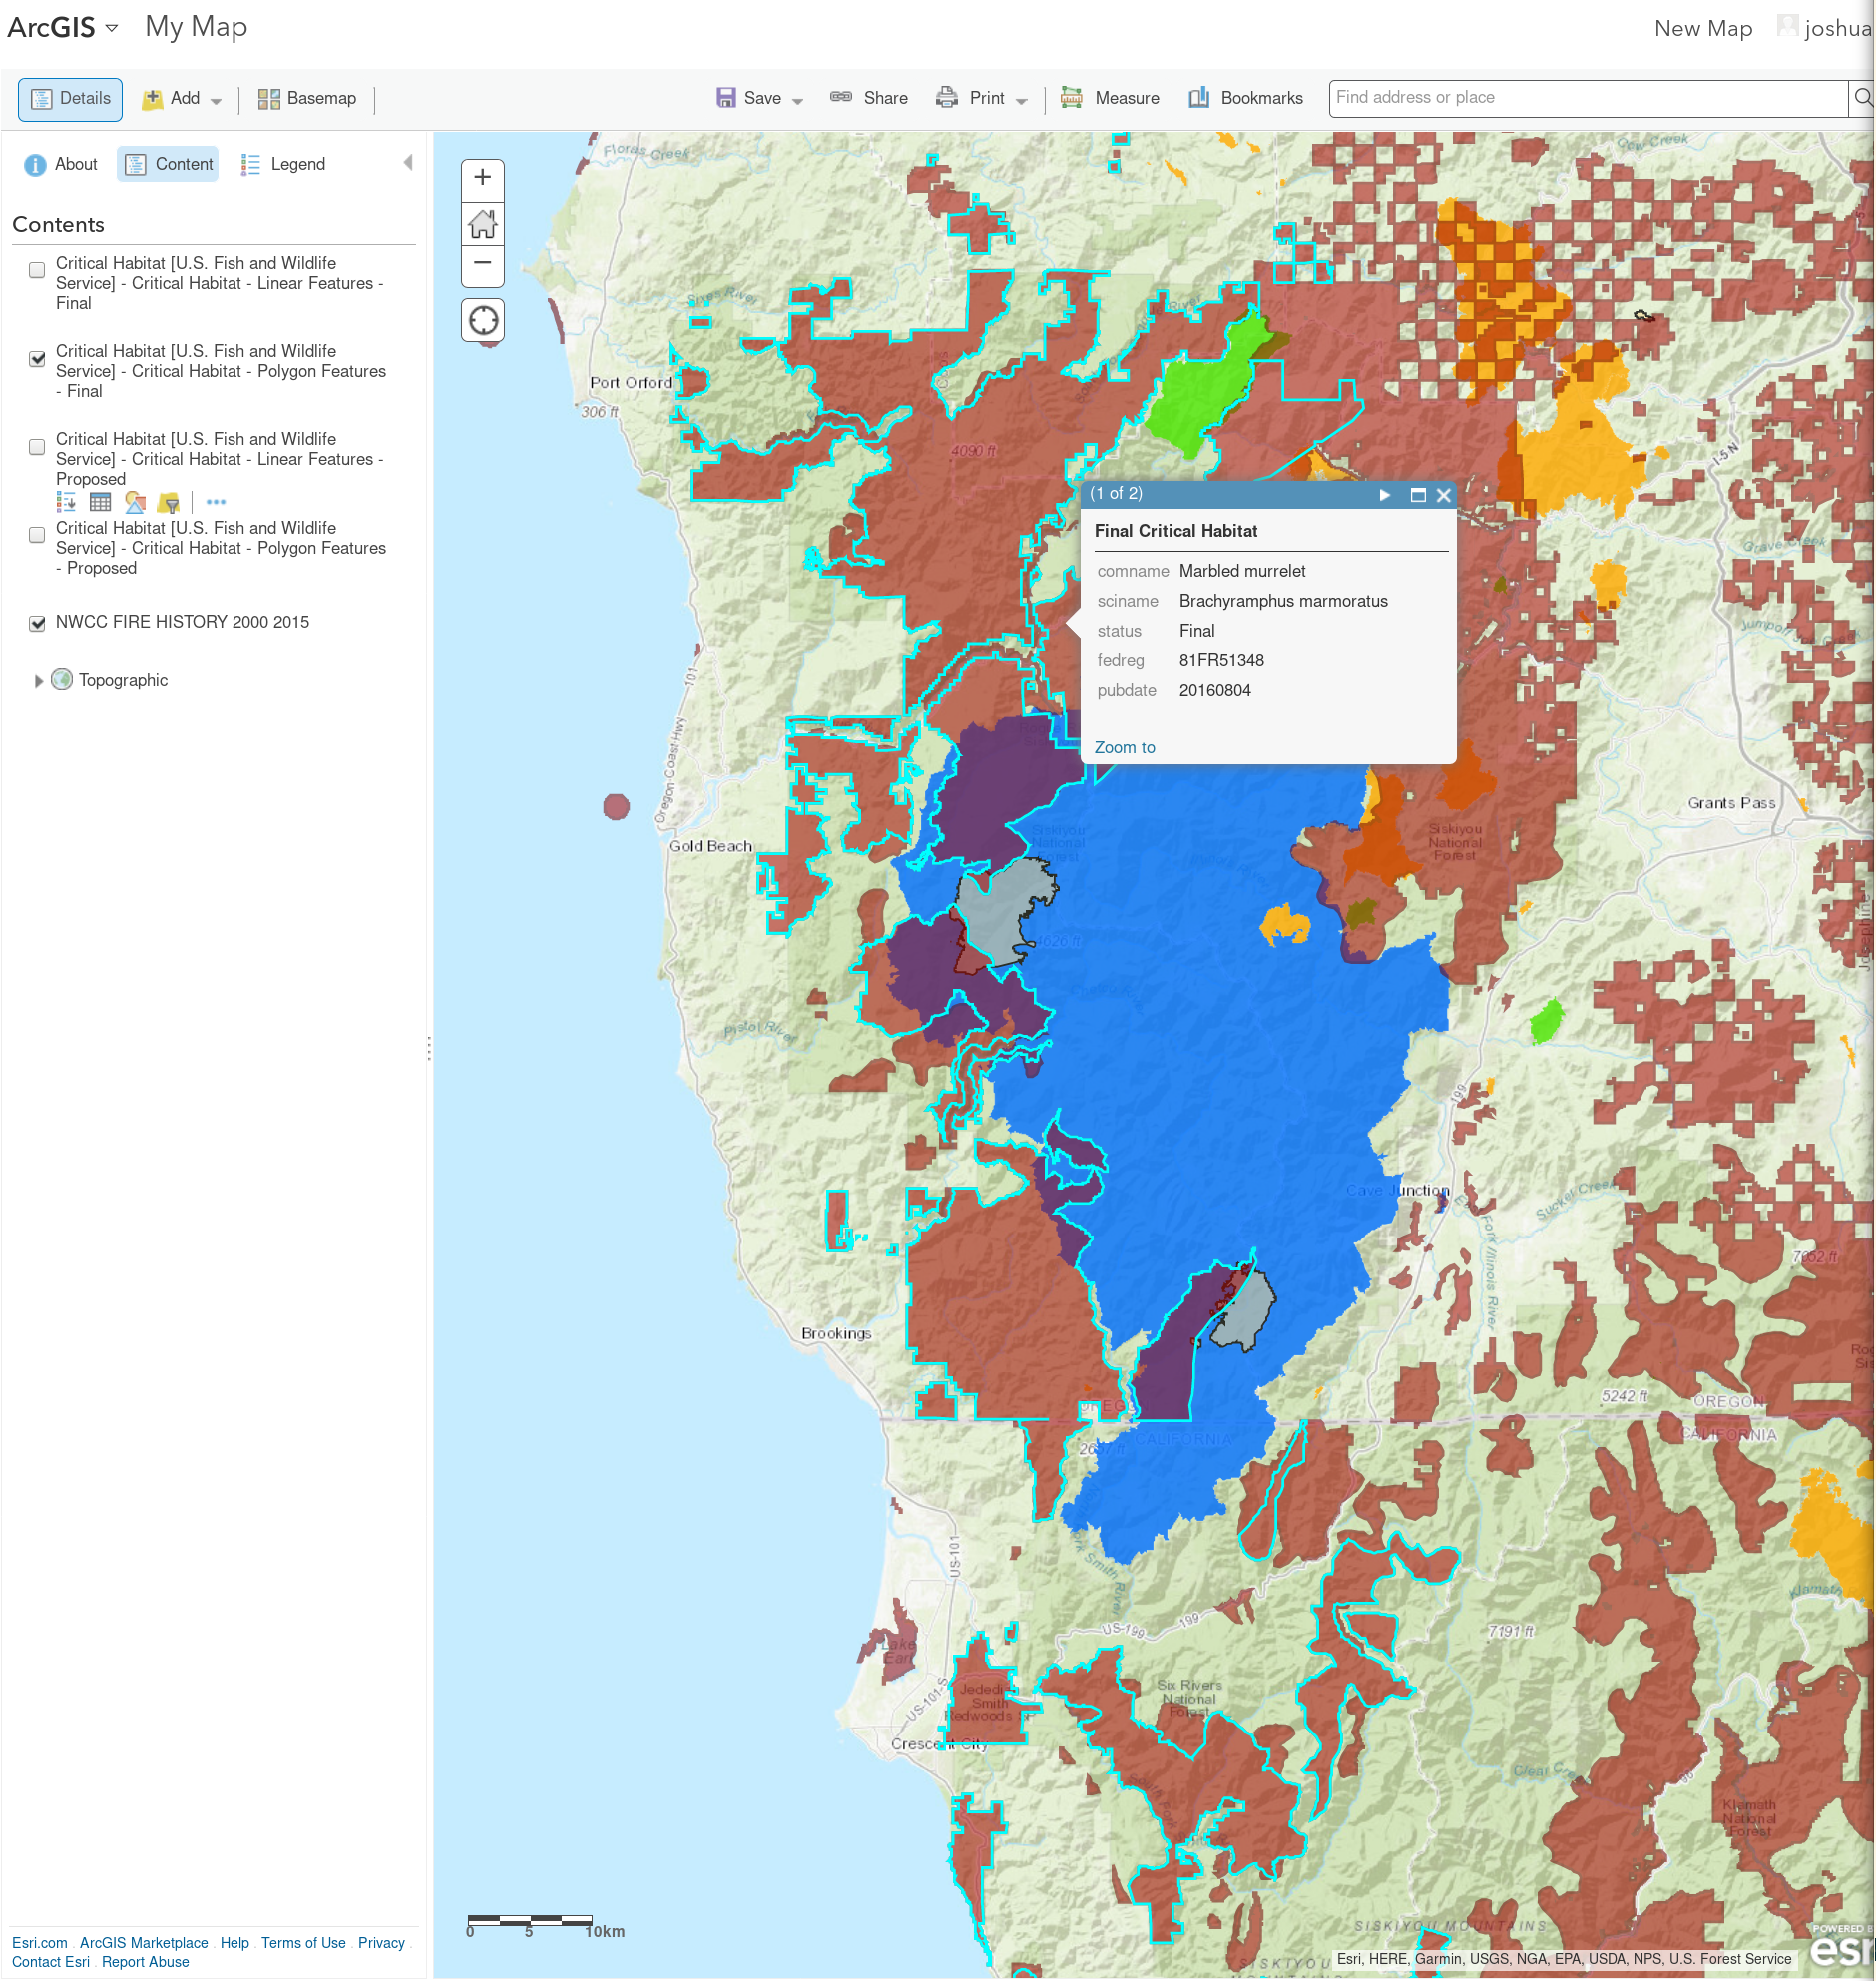
\includegraphics[width=\textwidth]{map}

\end{document}
